\chapter{Locomotion Controller Transfer from Virtual To Real World}
\section{Motivation}
Robotics and character animation share a common goal, to design locomotion controllers, the algorithmic ``brain'' that allow animated characters and robots to move naturally, robustly and efficiently in a complex dynamic environment. Despite this commonality, there is a gap between the state-of-the-art of these two fields. While in character animation, we have demonstrated that it is possible to control a full humanoid character to perform challenging locomotion tasks in a physically simulated environment, we have not yet seen any robots that have comparable capabilities. For example, controlling human walking is considered as a solved problem in character animation, but it is still an open research in robotics. In addition, we have demonstrated in the previous Chapters that with the powerful computational tools, controller can be optimized autonomously in a virtual environment. However, in robotics, designing controllers is still a challenging, trial-and-error process that is limited only to highly-specialized engineers. Can we extend the computational tools developed for character animations to robotics to close the gap between these two fields?

One major challenge to directly applying the methods we have developed to control robots is the Reality Gap: Controllers that work effectively for a virtual character in the simulation may perform poorly on a robot in the real environment. The most important factors that lead to the Reality Gap include hardware limitation, unmodelled dynamics, inaccurate physical properties, noise and latency. For example, the torque limits of the servos on the robot are seldom considered in animation applications. We also do not model the dynamics of the servos. Even though we often can acquire the physical properties, such as mass, center of mass and inertia, of a robot from its CAD files, they are usually inaccurate given the manufacturing error, assembly error and the cables that are not considered in CAD files. Furthermore, the noise in the environment and the latency in hardware communication also contribute to the Reality Gap.

To cross the Reality Gap and to design robotic controllers autonomously, we develop a system with three components, physical simulation, controller optimization and simulation calibration. We first build a physical simulation of articulated rigid bodies to model the dynamics of the robot and its environment. Different from the simulators used in animation, we incorporate the torque limits, servo dynamics, noise and latency measured from the robot experiments into our simulator. We then optimize a controller for a specific locomotion task in the physical simulation. However, if we apply this optimal controller directly to the robot, it will fail the task in the real world due to the Reality Gap. To solve this problem, we collect the real performance data, and use it to calibrate our physical simulator. We optimize a set of simulation parameters, including the mass, inertia, center of mass and actuator gains of the robot, to minimize the discrepancy between the simulation results and the collected real data. Through calibration, the simulator can capture the real world dynamics more faithfully. This calibrated simulator is used again in controller optimization to improve the quality of the controller. Depending on the task, it could take several iterations of simulation calibration and controller optimization to transfer the controller to the real robot. 

We evaluate our system in three locomotion tasks, rising from a leaning, sitting, or kneeling position to an erect stance. These motions are widely used in our daily life. Although most of us can perform them with ease, it is a big challenge for some elderly persons and patients with hamspring injuries. We choose to study these motions and synthesize them on robots due to these important health-care applications. One simple solution to achieve these tasks is to use static balance. The robot increases the area of the contact polygon by establishing more contact points, and then rises its body slowly while maintaining the COM within the contact polygon. We choose not to use this strategy because in real life, we human can perform these motions in a more agile fashion, and we hope that our controller can enable robots to demonstrate comparable agility. For this reason, our controllers will utilize impulsive actions and take advantage of the dynamic motion to rise. In addition, since one main contribution of our method is simulation calibration, to best test its effectiveness, we only use feedforward controllers in our evaluations. In contrast, if feedback controllers are used, the stability region of the task would be drastically increased, which makes the simulation accuracy less critical. Our results show that simulation calibration is effective. In most cases, only one iteration of calibration is needed to transfer the controller successfully to the real robot. Our system is able to design locomotion controllers autonomously, which work successfully both in the simulation and in the real world. 

\section{Overview}

\begin{figure}[!t]
  \centering
  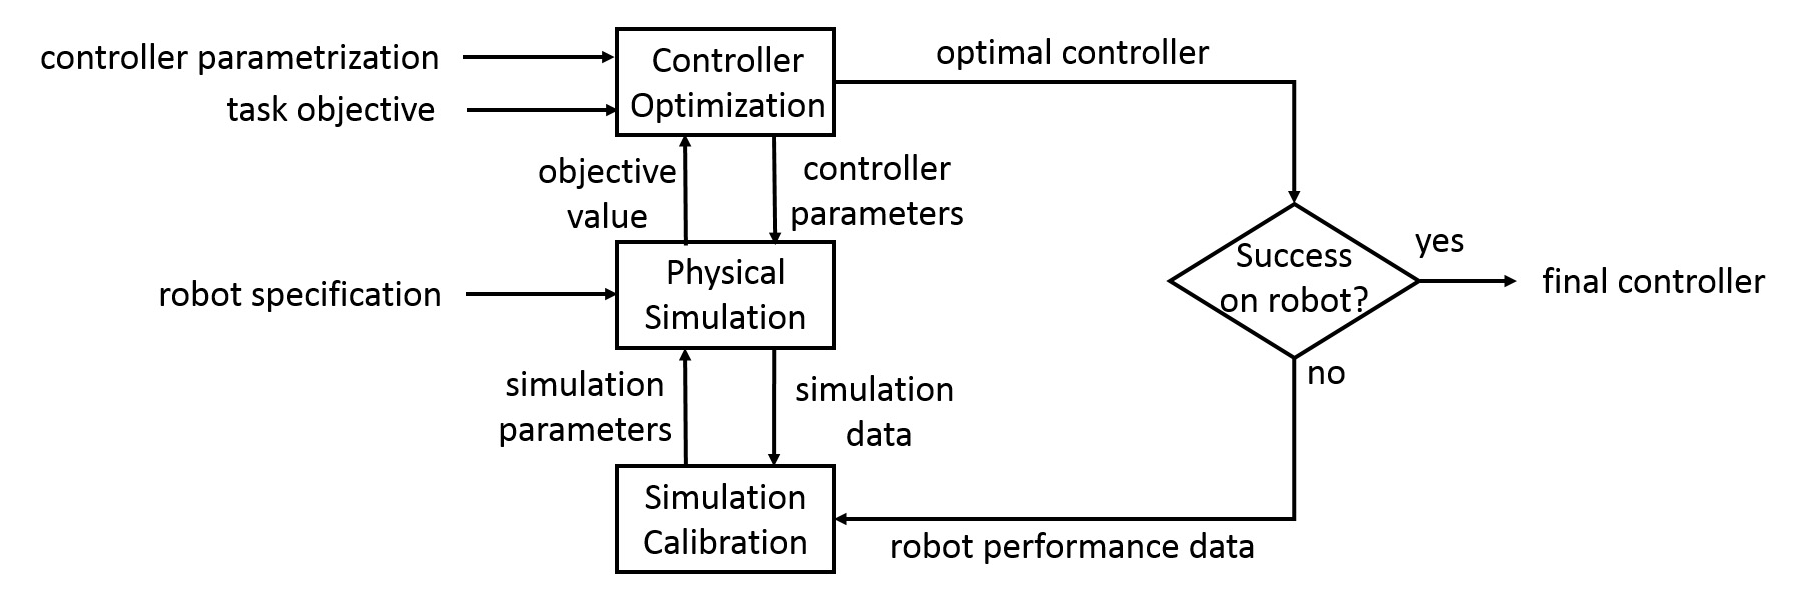
\includegraphics[width=6in]{figures/controllerTransfer}
  \caption{Overview of our algorithm.}
  \label{fig:controllerTransferOverview}
\end{figure}

We have designed a system that can automatically design locomotion controllers for robots (Figure~\ref{fig:controllerTransferOverview}). Given the specification of the robot, including its body shape, the physical properties of each body, and the types of joints, we build a physical simulation using Dynamic Animation and Robotics Toolkit (DART) \cite{dart:2012}, an open source articulated rigid body simulator. In addition, we also take into consideration the torque limits, servo gains, noise and latency, which are not modeled in DART. The controller optimization subsystem runs thousands of simulations to search for the optimal controller to minimize the task-related objective function. We then test this optimal controller on the robot. If the robot successfully completes the task, a working robotic controller is found and our algorithm terminates. Otherwise, we record the robot performance data and feed it into the simulation calibration subsystem. Simulation calibration runs another optimization, which searches for the optimal simulation parameters to minimize the discrepancy between the performance data from the simulation and that from the robot experiments. The loop of controller optimization and simulation calibration is performed iteratively until the controller works successfully on the real robot. In the next three sections, we will delve into the details of these main components of our system, physical simulation, controller optimization and system calibration.

\section{Physical Simulation}
\section{Controller Optimization}
\section{System Calibration}
\section{Results}
\section{Discussion}
